\documentclass[conference]{IEEEtran}
\IEEEoverridecommandlockouts
% The preceding line is only needed to identify funding in the first footnote. If that is unneeded, please comment it out.
\usepackage{cite}
\usepackage{amsmath,amssymb,amsfonts}
\usepackage{algorithmic}
\usepackage{graphicx}
\usepackage{textcomp}
\usepackage{xcolor}
\def\BibTeX{{\rm B\kern-.05em{\sc i\kern-.025em b}\kern-.08em
    T\kern-.1667em\lower.7ex\hbox{E}\kern-.125emX}}
\begin{document}

\title{Term Project Part-2 Report\\
{\footnotesize \textsuperscript{}}
\thanks{}
}

\author{\IEEEauthorblockN{Beyza BUTUN
\IEEEauthorblockA{2171411} \\
}

\IEEEauthorblockN{ Soner DURMAZ}
\IEEEauthorblockA{2171551 \\
}
}

\maketitle


\section{Introduction}
Before writing the code, we designed our project to receive an input from the file which has 5MB size(5000000 characters in this file), and to send it to destination. To be able to that, we thought the source as the client and server which use TCP and also we thought broker as the client and the server which use TCP and UDP. Finally, we thought destination as the client and the server which use UDP. Moreover, before the writing part, we thought about how we can add an IP to a router table. After that, we started programming part.

\section{Programming Part}

\subsection{source.py}
First of all, we added 800 characters which has been taken from the input.txt file into the messageS array which we had created. These are the messages that we aim to send to the destination.\\

After that, we created checksum function(chksum) to calculate checksum of the characters which is in the input. This function converts the characters in the data to their ASCII code, then it finds sum of them and take its NOT. We used this function to detect the bit errors.\\

Then we created signal$\_$handler function to halt the program.\\

After that, to be able to do pipelining and multihoming, we used thread mechanism. For that, we created 3 functions (sender1, sender2, sender3) to send messages to the different ports(25698,25798,25898) of brokers. We used TCP to send messages, because TCP provides us congestion control mechanism. By using that, we prevented from congestion. In these functions, we created client socket, and connected it to the one of the broker IPs and ports. Then we checked whether it exceeded the windows size or not, and we checked whether this message has sent before or not.To check whether the message has sent, we created an array named DataSended. When source receive the ACK messages, we wrote 1 into its index. Then, If it didn't exceed windows size, and it has not sent before, we created a new message by adding its checksum and index into it. After that, we made source send this message to the broker.Then, we did close the client socket. Sender1, sender2 and sender3 do the same thing, but they send messages to the different IPs and ports of the broker.\\

Then, we created timer function. Once in 1.5 second, we added the index of the message sended to the beginning of the windows size(cwndLocation). Then we updated the end of the windows size.\\

After that, to receive ACK messages from broker, we wrote ackReceiver, ackReceiver2 and ackReceiver3 functions. For each function, first, we created a connection socket, after we had created server sockets and we did receive ACK message from broker. We did receive the ACK messages from the ports 16000, 16001 and 16002 of the broker. The ACK message is actually the index of the message. So, first we assigned 1 to the index of the message in DataSended array. After that, if the index of the message(ACK message) is equal to the index of the first message which the source has not received its ACK message, we changed the beginning of the windows size. We assigned the next index which the source has not received its ACK message yet to the beginning of the windows size(cwndLocation). Whenever we take the ACK message, we increased the count. After that, we close the connection socket. 

For pipelining and multihoming, we used Thread mechanism. Then we started all functions by using start() function. By doing these, we made the functions work synchronically. It was important for us to halt the program. To do that, we use daemon. Because if thread.daemon = True is specified for python thread, then the program will halt immediately when only the daemon is left. We used this feature.\\

In the final while loop, we checked whether all messages's ACK has received or not. If it has, we called the signal function, and halt the program.

\subsection{broker.py}
In the broker part, we created three functions which are named receiver1, receiver2 and receiver3 to receive messages from the source, and send them to destination. To receive the messages, we used TCP, because it has congestion control mechanism. These three functions receive messages from different ports of the source. After they receives messages, to send the messages to the destination by using UDP we created client socket. Then, when we divide the index of the message by 3, if the remainder is zero, we made the broker send the message to 10.10.3.2 with the port 25699, if it is one, we made the broker send the message to 10.10.5.2 with the port 25799, and finally if it is two, we made the broker send the message to 10.10.5.2 with the port 25899. These are destination's IPs and ports. \\

After that, to receive the ACK messages from the destination, we created three functions which are named ackReceiver, ackReceiver1 and ackReceiver2. To be able to do that, we created server socket, and from this socket we received the ACK messages from the destination's port 17000, 17001 and 17002. To make the broker send ACK messages to the source by using TCP, we created client socket, and we made the broker send these messages to the source. This ACK messages is sent to the source IP 10.10.1.1 with the ports 16000, 16001 and 16002. After that, we closed the client sockets. \\

To do the all receiving and sending works synchronically, we use threading mechanism again. Finally, we started all functions simultaneously.

\subsection{Routing Table}
To be able to send messages from broker to the destination, we used routing table. We added the destination IPs to the table with these commands:\\
route add -net 10.10.3.2 netmask 255.255.255.254 gw 10.10.2.2 dev eth2\\
route add -net 10.10.5.2 netmask 255.255.255.254 gw 10.10.4.2 dev eth1 \\
In these commands, gateway is the IPs of the routers.\\

Then, to be able to send messages from the destination to the broker, we used again routing table. We added the broker IPs to the table with these commands:\\
route add -net 10.10.2.1 netmask 255.255.254.0 gw 10.10.3.1 dev eth2\\
route add -net 10.10.1.2 netmask 255.255.255.254 gw 10.10.5.1 dev eth2\\
In these commands, gateway is the IPs of the routers.

\subsection{destination.py}
In destination part, first we created sum function. This function converts the characters in the data to their ASCII code, then it finds sum of them. We use this function to check the bit errors. \\

After that, we created signal$\_$handler function to halt the program.\\

Destination receives the messages from broker with UDP, and send the ACK messages of these messages to the broker by using UDP again. To be able to do that, we created three functions which is named Receiver, Receiver1 and Receiver2. First these functions receives the messages and after it checks their checksum and receiving situation which we will express later, the destinations sends them the messages' ACK to the broker. \\

In each function, first we created a server socket to receive messages from the broker with the ports 25699, 25799 and 25899. From this server socket, we received the messages. First, we seperated the message, because in the source we had added the checksum and index of the message to the message. So, after that, we had the message, checksum of the message and the index of the message. \\

After that we checked whether this message is the correct message or not by using checksum of the message and the sum function. If their sum is equal to -1, this means it is the correct message. In the beginning of the code, we had created RecInd array which shows whether a message has received before or not. \\

If the message is correct and the message has not received before, we assigned the message to the the index in DataReceived array. After that, we assigned 1 to the index in the RecInd array to show that the message had received. Then we incresed the counter. \\

If the message is correct but the message has received before, and the other case, we send the message to the broker IP 10.10.1.2 and 10.10.2.1 with the ports 17000, 17001 and 17002. After that, we closed client sockets.
Because we used the target mechanism in destination too, we started all the functions simultaneously. \\

Again to halt the program we used daemon mechanism. When the counter is 6250, which means when the all messages has received, after waiting 3 seconds, we called the signal function, then it halts the program.
However, before halting the program, we did create a file named output.txt, and sent the datas received to this file.

\section{Graph}
Packet Loss:
\begin{verbatim}
x=[0.5,10,20];
y=[80.28,771.1,2316.33];
e=[0,0,0];
errorbar(x,y,e);
xlabel('packet loss percentage');
ylabel('file transfer time(sec)');
title('packet loss percentage vs file transfer time');
print('graph.png')
pause;
\end{verbatim}

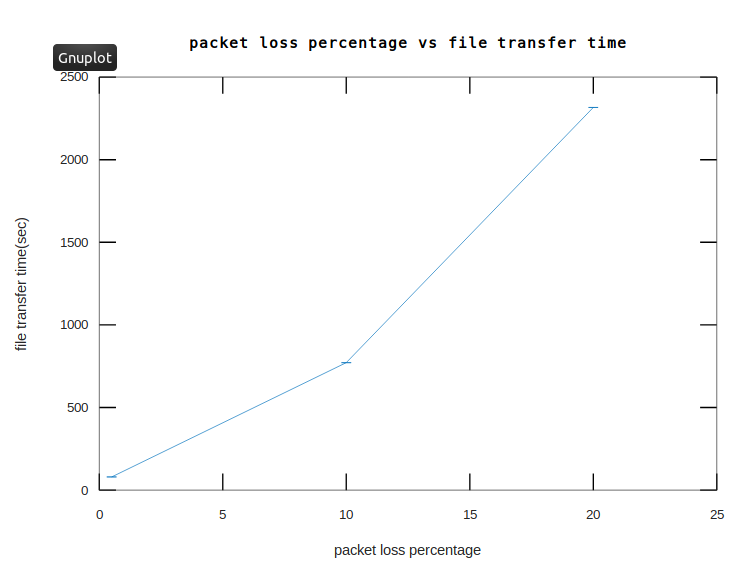
\includegraphics[width=9cm,scale=0.25]{loss.png}\\[0.1cm]
\\
\\

Since our file transfer time is huge, we can think that our congestion control is bad. We couldn't calculate our standard deviation because to calculate it we had to transfer the file many times but when we consider our base file transfer time it may take a couple of day. Also we can see that our file transfer time is going up while packet loss percentage goes up, linearly.
\\
\\
Corruption: 

\begin{verbatim}
x=[0.2,10,20];
y=[72.51,692.74,2003.27];
e=[0,0,0];
errorbar(x,y,e);
xlabel('corruption percentage');
ylabel('file transfer time(sec)');
title('corruption percentage vs
file transfer time');
print('graph.png')
pause;
\end{verbatim}

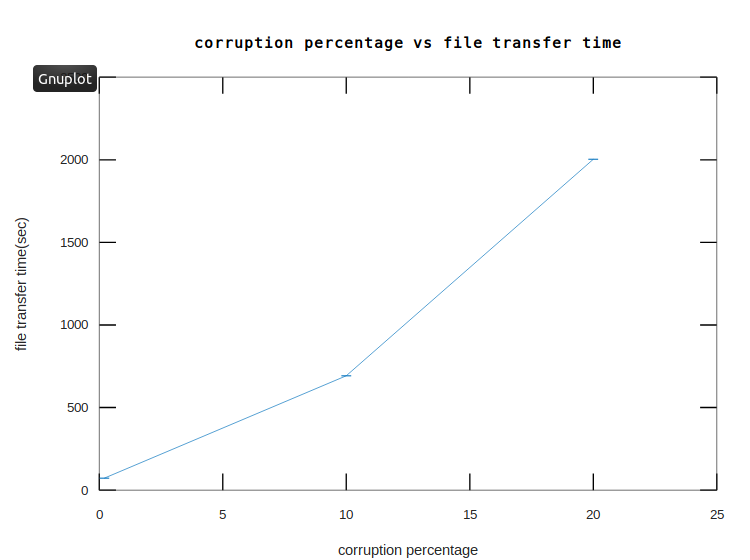
\includegraphics[width=9cm,scale=0.25]{corrup.png}\\[0.1cm]

Since our file transfer time is huge, we can think that our congestion control is bad. We couldn't calculate our standard deviation because to calculate it we had to transfer the file many times but when we consider our base file transfer time it may take a couple of day. Also we can see that our file transfer time is going up while corruption percentage goes up, linearly.
\\
\\
Reordering:

\begin{verbatim}
x=[1,10,35];
y=[58.64,60.23,157.02];
e=[0,0,0];
errorbar(x,y,e);
xlabel('reordering percentage');
ylabel('file transfer time(sec)');
title('reordering percentage vs
file transfer time');
print('graph.png')
pause;
\end{verbatim}

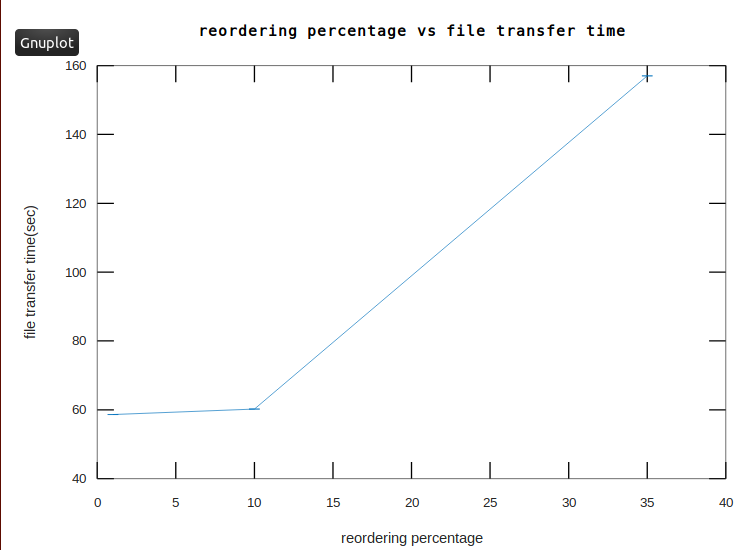
\includegraphics[width=9cm,scale=0.25]{reorder.png}\\[0.1cm]

Since our file transfer time is huge, we can think that our congestion control is bad. We couldn't calculate our standard deviation because to calculate it we had to transfer the file many times but when we consider our base file transfer time it may take many hours. Also we can see that our file transfer time is going up while reordering percentage goes up, linearly.
\\
\\
\\
\\
\\
\\
\\
\\
\\
\textit{During the term project, we designed and implemented all parts together. }


\end{document}

